\section{Boundary condition three: production and recompute}
\label{sec:production}

% source: PAPER_SKELETON Sec 6; EVIDENCE_lineage_boundaries L-prod / L-lab / L-rec.

\paragraph{Absorption is a property of in-stream continuation, and this
part corroborates prior work.} The same audited-false plant that Qwen2.5-7B
absorbs at 0.86 while continuing its own stream is absorbed at about 0.15
when the identical content is re-presented as a fresh chat turn, and at
about 0.00 once restatement of the plant is suppressed; closure-valid
completion rises correspondingly as the model re-plans through the true
chain.
% source: EVIDENCE_lineage_boundaries L-prod.1 (0.863 -> 0.150 -> 0.000; valid 0.093->0.85->1.00)
A diagnostic shows the two failure modes trade off, so this is not fixable
by prompt tightening. We frame this in-stream-versus-fresh-turn boundary as
corroboration of concurrent work on the self-correction blind spot
\citep{tsui2025blindspot, chen2026selfcorrection}, not as a discovery. Our
delta over that work is a silent-reuse measure that answer-naming judges
miss, a near-total magnitude, 0.86 to about zero rather than a few points of
dilution, and an audited-logic substrate.
% source: EVIDENCE_lineage_boundaries L-prod.1 MANDATORY framing; STYLE_SHEET production boundary

\paragraph{Re-read rejection is training-recipe-bound, a lab-level split
rather than a capability ladder.} Under an identical prefill harness, the
current Anthropic chat lineage rejects every audited plant, with
derivational injection-dependence of 0.000 in all twelve cells for each of
two models, including the very cell where Qwen absorbs at 0.86, while the
current OpenAI lineage still absorbs.
% source: EVIDENCE_lineage_boundaries L-lab.2 (0.000 all 12 cells x2); L-lab.1
In the one directly comparable format, instruct-mode on each model's own
traces with audited-false plants, echo-corrected reuse of a false category
is 0.58 for gpt-4.1 and 0.01 for claude-sonnet-5, spanning the open-weights
anchor of 0.35 in between.\pending{add Self-Attribution Bias
2603.04582 and Cross-Context Review 2603.12123 as stubs when this sentence
is wired in Sec~9.}
% source: EVIDENCE_lineage_boundaries L-lab.1 (gpt-4.1 0.580, sonnet-5 0.010, Qwen 0.350)
The oldest generation point we could run under true text completion,
2023-era gpt-3.5-turbo-instruct, is the deepest absorber measured anywhere,
at echo-corrected reuse 0.57, giving the lineage a non-monotone shape that
complicates any clean training-recipe or monotone-compute story.
% source: EVIDENCE_lineage_boundaries L-lab.4 (gpt-3.5-instruct reuse 0.571)
We keep this arm descriptive and single-seed, and we scope ``Anthropic
best'' to the re-read prefill regime, because those same models fail in a
monitoring regime studied elsewhere.\pending{cite Self-Attribution Bias
2603.04582 here once abs-verified (it shows Anthropic models fail in the
monitoring regime).}
% source: EVIDENCE_lineage_boundaries L-lab.1 caveat; RELATED_WORK_MAP P5 (Self-Attribution Bias)

\paragraph{But there is a universal recompute boundary: no model
re-verifies a computed value.} In a program-execution regime we can
separate a falsehood whose true value can be \emph{re-read} from an earlier
line from one whose true value must be \emph{re-computed}. The two frontier
Anthropic models reject re-readable falsehoods near totally, at 0.00 to
0.22, yet absorb a five-operation recompute chain at 1.00, indistinguishable
from Qwen; a one-operation recompute is already absorbed at 0.98 to 1.00.
% source: EVIDENCE_lineage_boundaries L-rec.1 (deep_kc5 1.000/1.000; onehop_kc1 1.000/0.983; opfree_kr1 0.043)
No model we tested re-verifies a value it must recompute. We distinguish a
final-answer flip from re-derivation of the specific computed intermediate,
so this is not contradicted by math self-correction results, and we scope
the universality to the three models actually run on those cells until a
broader run lands.
% source: EVIDENCE_lineage_boundaries L-rec.1 MANDATORY framing; \pending{E2 EXPG-FULL is optional for TMLR}
This recompute boundary is the one result in the paper that holds across
scale, family, and lineage.

\paragraph{A conjecture from the earlier draft is now confirmed.} The
earlier workshop draft conjectured that absorption is carried by
continuation pressure rather than by the content of the plant. The bridge
experiment above confirms it, as a continuity asset rather than a
retraction: suppressing in-stream restatement removes absorption entirely.
% source: PAPER_SKELETON 6.6; EVIDENCE_lineage_boundaries L-prod.1

\begin{figure}[t]
\centering
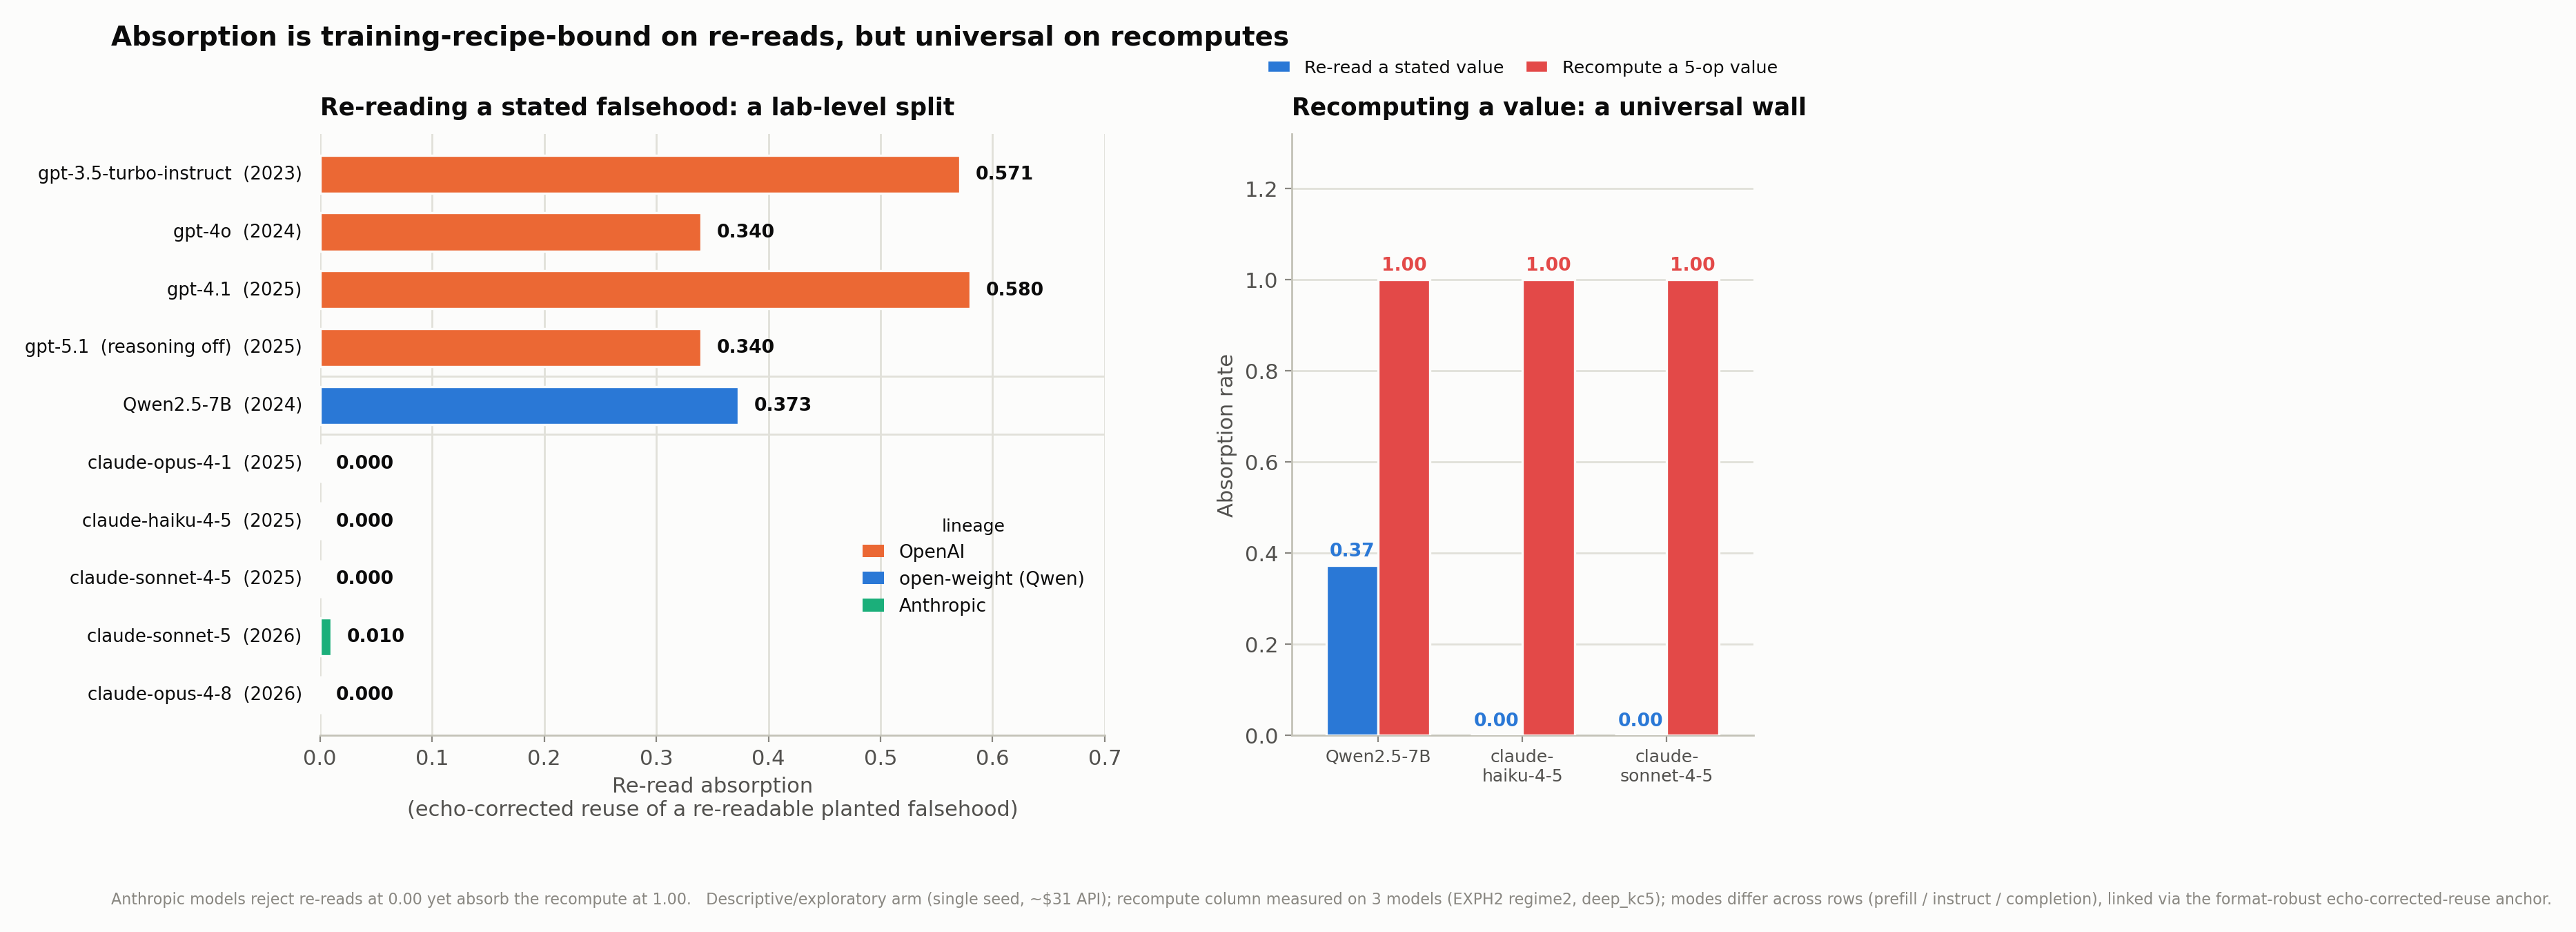
\includegraphics[width=0.92\textwidth]{figures/fig_d_lineage_recompute.png}
\caption{\textbf{Lineage split on re-reads; a universal wall on recomputes.}
Left: echo-corrected reuse of a re-readable planted falsehood is
lab-shaped and non-monotone in capability, with 2023 gpt-3.5-instruct
(0.57) and gpt-4.1 (0.58) the deepest absorbers, the open anchor at 0.37
(the prefill-locked format value; the same Qwen comparator is 0.350 in the
instruct format used for the cross-lab comparison in the body text),
and every Anthropic model near 0.00. Right: on recomputes there is no
split, the two Anthropic models that reject re-reads at 0.00 still absorb a
five-operation recompute at 1.00. This whole panel is descriptive,
single-seed, roughly \$31 of API; rows in the left panel use different
modes (prefill / instruct / true completion) and are linked only through
the format-robust echo-corrected-reuse anchor, so read it as a gradient,
not one controlled ladder. Never read it as ``Anthropic checks every time''
(supported claim: rejects every audited falsehood, reuse 0.000) or
``gpt-4.1 never checks'' (only its reuse rate 0.58 is on record).}
% source: figures/FIGURE_CAPTION_PLANS Fig D
\label{fig:lineage}
\end{figure}
